\subsection{Pengujian Citra \emph{Depth Camera} pada \emph{Real Robot}}
\label{subsec:citradepthrobot}

Sama seperti pada pengujian sebelumnya di bagian \ref{subsec:citradepthsimulasi},
  pengujian citra \emph{depth camera} pada \emph{real robot} dilakukan dengan menjalankan dua buah \emph{image viewer node} untuk melihat hasil penerimaan data citra berwarna dan citra kedalaman.
Hanya saja, sebagai ganti dari \emph{node} \lstinline{/depth_camera_plugin} yang ada di simulasi,
  data citra berwarna dan citra kedalaman yang digunakan akan berasal dari \emph{Kinect2 node}.
Seperti yang dapat dilihat pada gambar \ref{fig:rosgraphdepthcamera},
  \emph{node} \lstinline{/kinect2} akan mengirimkan \emph{topic} \lstinline{/kinect2/depth/image_raw} yang berisi citra kedalaman ke \emph{node} \lstinline{/image_viewer_2},
  serta \emph{topic} \lstinline{/kinect2/image_raw} yang berisi citra berwarna ke \emph{node} \lstinline{/image_viewer_1}.

\begin{figure}[ht]
  \centering
  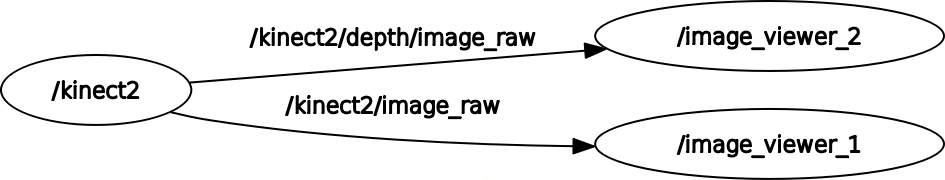
\includegraphics[width=0.95\textwidth,keepaspectratio]{gambar/rosgraph-depth-camera.png}
  \caption{Relasi antar-\emph{node} dari pengujian citra \emph{depth camera} pada \emph{real robot}.}
  \label{fig:rosgraphdepthcamera}
\end{figure}

Hasilnya, kedua \emph{image viewer node} tersebut akan menampilkan citra yang dikirim oleh \emph{Kinect2 node}.
Seperti yang dapat dilihat pada gambar \ref{fig:depthcamerarobot},
  gambar pertama menampilkan citra dari ruang lab komputer secara berwarna,
  sedangkan gambar kedua menampilkan citra dari ruang lab komputer secara hitam putih.
Berbeda dengan hasil yang didapatkan di simulasi, pada pengujian ini,
  citra kedalaman yang didapatkan memiliki hasil yang sangat terang.
Hal ini terjadi karena pendeknya jangkauan yang dimiliki Kinect V2, yakni hanya sejauh 4.5 meter.

\begin{figure}[ht]
  \centering
  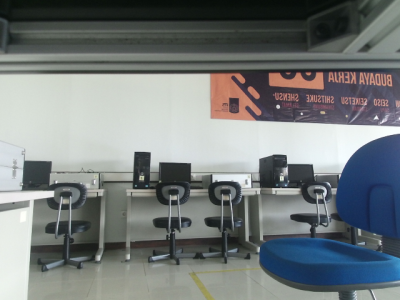
\includegraphics[width=0.45\textwidth,keepaspectratio]{gambar/citra-depth-camera-rgb-robot.png}
  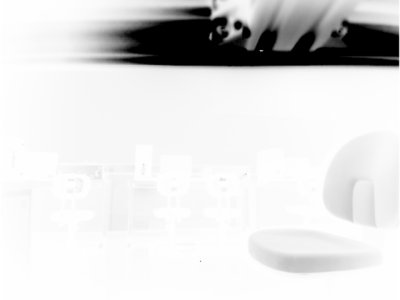
\includegraphics[width=0.45\textwidth,keepaspectratio]{gambar/citra-depth-camera-depth-robot.png}
  \caption{Perbandingan hasil tangkapan citra berwarna dan citra kedalaman pada \emph{real robot}.}
  \label{fig:depthcamerarobot}
\end{figure}
